\chapter{Calculating a stitched spectrum from time series}
\label{App:stitch_spec}

Many existing programs and scripts exist that compute the fast Fourier transform (FFT) and corresponding spectral density of an input time series. However, for a number of reasons we have found it advantageous to compute several FFT's from the time capture and to ``stitch'' them together to represent the spectrum. In this Appendix, we review our algorithm to compute the FFT's and to stitch them into a single spectrum.

Given an input time series, sampled at a frequency $1/\Delta t$ and consisting of $N$ points of amplitude $y_j$ ($j \in \{1, 2, 3, \ldots\}$), the FFT is defined as
\begin{align}\label{eqn:defFFT}
Y_k = \sum_{j=1}^N y_j \omega_N^{(j-1)(k-1)},
\end{align}
where $\omega_N = \exp[-2\pi i/N]$ is an $N^\text{th}$ root of unity. In general, the FFT algorithm works best when $N$ is a power of 2; if it is not, $y_j$ is usually padded with zeros until its length is a power of 2. Because $y_j \in \mathbb{R}$, $Y_k$ is symmetric ($Y_{k} = Y_{N-k+2}^*$ for $k \ge 2$) and the power spectral density $S_k$ can be written as
\begin{align}
S_k =
  \begin{cases}
   \frac{\Delta t}{N} |Y_1|^2 &\text{if } k = 1 \\
   2\frac{\Delta t}{N} |Y_k|^2 &\text{if } k \in \{2, 3, 4, \ldots N/2 + 1 \}
  \end{cases},
\end{align}
which is defined at frequencies $f_k = (k-1)/N \Delta t$, where $k \in \{1, 2, 3, \ldots N/2 + 1 \}$.

One can compute a single FFT of the entire time capture ($N = \Ntc$). However, this technique leads to a spectrum that appears extremely noisy; that is, the difference between the spectral density at adjacent frequencies is of the order of the spectral density itself, regardless of the length of the time capture. This property can be understood as follows. At any particular frequency, $S_k$ is the sum of the squares of the real and an imaginary components of $Y_k$, which are independent for random noise. Therefore, $S_k$ follows a Chi-squared distribution with two degrees of freedom ($S_k \sim \chi_2^2$). A property of the $\chi_2^2$ distribution is that the variance $\sigma^2$ is equal to its mean $\mu$ squared. Therefore, $\sigma^2(S_k) = \mu^2(S_k)$ so that the spread of spectral densities is relatively large and the spectrum appears noisy. A longer time capture increases $\Ntc$, which in turn increases the frequency resolution---the width of the frequency bins $df = 1/N\Delta t = 1/\Ntc\Delta t$---but does not decrease $\sigma^2(S_k)$.

To reduce the apparent noise in the spectrum, it is typical to introduce some form of averaging. A popular method is to split the time capture into $\Navg$ equivalent-length segments, computing the FFT for each segment and averaging the spectral densities to form a single averaged spectrum. In other words,
\begin{align}\label{eqn:Sk_averaged_def}
S_k = \frac{1}{\Navg} \sum S_{k,n},
\end{align}
where $S_k$ is now an averaged spectral density and $S_{k,n}$ is the spectral density at $f_k$ of the $n^\text{th}$ time segment. In this case, $S_k$ obeys the central limit theorem and, for sufficiently large $\Navg$, is normally distributed with a variance that scales as $1/\Navg$. Since
\begin{align}\label{eqn:df_Navg_def}
df = \frac{\Navg}{\Ntc}\frac{1}{\Delta t},
\end{align}
we see that there is a tradeoff between high frequency resolution and low variance of the spectral density. Because the lowest frequency of the spectrum (zero frequency excluded) is equal to $df$, the tradeoff is equivalently between a spectrum that extends low in frequency and one that is highly averaged.

\begin{figure}
\centering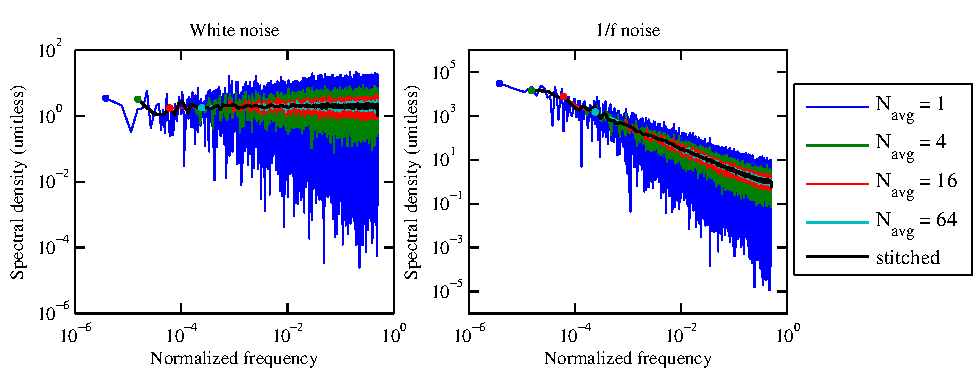
\includegraphics[width=6.5in]{stitch_spec/white_pink_noise_spectra}\\
\caption[Spectral density of white and $1/f$ noise]{Spectral densities of (a) white and (b) $1/f$ noise vs frequency, normalized to $1/dt$. Spectra are computed from randomly generated time series with $\Ntc = 2^{18}$ for varying $\Navg$. Colored dots are plotted to highlight the lowest frequency of each spectrum. In addition, a stitched spectrum with $\Navg = [4, 16, 64, 256]$ and $\fcut = (0.5/50) * [1/2^6, 1/2^4, 1/2^2]$ is shown. [@@@ Add subfigure labels].}
\label{Fig:white_pink_noise_spectra}
\end{figure}

To circumvent this tradeoff, we observe that, for our application, a high frequency resolution is not necessary at high frequencies. Similarly, at low frequencies we can tolerate relatively few averages, which in turn gives us high frequency resolution. This situation suggests that we compute an averaged FFT with relatively low $\Navg_\text{,min}$ for low frequencies and large $\Navg_\text{,max}$ for high frequencies. The spectra generated by using different values of $\Navg$ can be stitched together at some intermediate frequency $\fcut$. If $\Navg_\text{,min}$ and $\Navg_\text{,max}$ are significantly different, intermediate values of $\Navg$ can be used as well. The standard 1~hr time capture we acquire during noise measurements consists of $3200*1024 = 3,276,800$ points, sampled at 1024~Hz. To compute the spectral density, we use $\Navg = [3, 12, 50, 200, 800, 3200]$ to generate 6~FFT's, which we stitch together at the frequencies $\fcut = [1/2^{10}, 1/2^8, 1/2^6, 1/2^4, 1/2^2]*(512~\text{Hz}/50) = [0.01, 0.04, 0.16, 0.64, 2.56]$~Hz.

Figure~\ref{Fig:white_pink_noise_spectra} shows the spectral density of white and $1/f$ noise computed in a variety of ways from two separately randomly generated time series. For unstitched spectra, we see that the variance in spectral density points decreases as $\Navg$ increases. Correspondingly, the lowest frequency to which the spectral density extends, represented by the colored dots, also increases with $\Navg$. The stitched spectrum, however, extends to a low frequency while maintaining a low variance at high frequency points.

\begin{figure}
\centering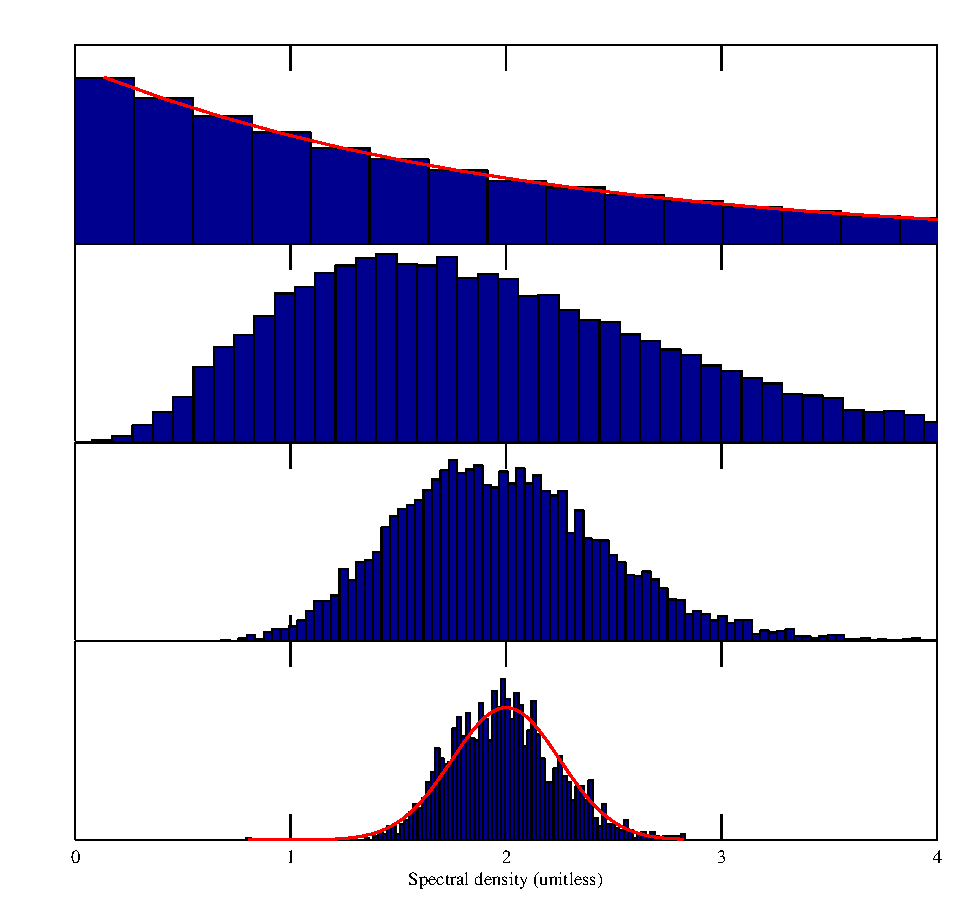
\includegraphics{stitch_spec/noise_histograms}\\
\caption[Histograms of white noise]{Histograms of white noise from Fig.~\ref{Fig:white_pink_noise_spectra}(a) for (a) $\Navg = 1$, (b) $\Navg = 4$, (c) $\Navg = 16$, and (d) $\Navg = 64$. The probability distributions fit (a) a $\chi_2^2$ distribution (solid red line) and (d) a normal distribution with standard deviation that scales as $\Navg^{-1/2}$ (solid red line). [@@@ Add ylabel 'Normalized counts', legend, subfigure labels].}
\label{Fig:noise_histograms}
\end{figure}

In Fig.~\ref{Fig:noise_histograms} we histogram the spectral densities of the white noise shown in Fig.~\ref{Fig:white_pink_noise_spectra}(a) to illustrate the effect that $\Navg$ has on the variance. As mentioned earlier, the spectral densities generated from a single FFT are distributed following a $\chi_2^2$ distribution, as shown in Fig.~\ref{Fig:noise_histograms}(a). As $\Navg$ increases, the distribution of spectral densities, which are now averaged from several FFTs, approaches a normal distribution with a standard deviation that scales as $\Navg^{-1/2}$ according to the central limit theorem. For $\Navg = 64$, the agreement with the normal distribution is good [Fig.~\ref{Fig:noise_histograms}(d)]. The same phenomenon 